
\chapter{\label{reseau}Les réseaux de neurones}

Dans cette partie, nous présentons de manière simplifiée les réseaux de neurones 
et comment les utiliser pour résoudre notre problème de classification.
Ce chapitre s'inspire fortement de \textit{Neural Networks and Deep Learning}\cite{neuralnetworksanddeeplearning} 
et en reprend les notations.


\section{Le modèle du perceptron}



\begin{definition}[Fonction de Heaviside]
On appelle fonction de Heaviside la fonction $H$ définie de $\mathbb{R}$ dans $\{0, 1\}$ par :
\[
H(x) = 
\begin{cases}
 1, \text{ si } x \geq 0 \\
 0, \text{ sinon.} 
 \end{cases}
\]
\end{definition}

\begin{figure}[h]
  \centering
  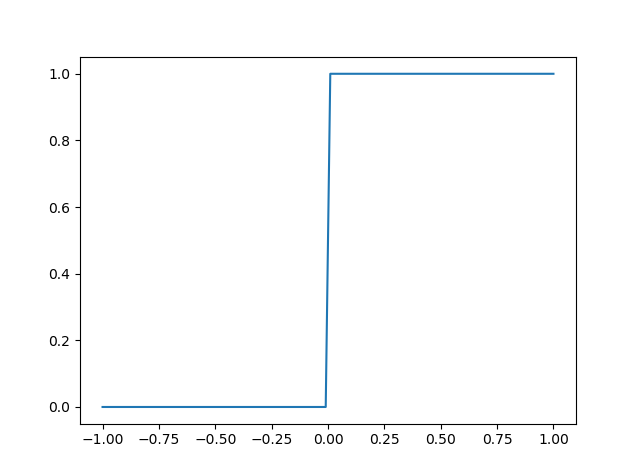
\includegraphics[scale=0.5]{assets/heaviside}
  \caption{La fonction échelon unité, ou fonction de Heaviside.}
  \label{fig:heaviside}
\end{figure}

Le but du perceptron est de modéliser le comportement du neurone biologique. 
Ce dernier est stimulé par des signaux qui lui parviennent par ses dendrites et, si 
la stimulation est suffisament importante, renvoie un signal à d'autres neurones au travers de son axone.

En notant $x_1, x_2, \dots, x_n$ ces stimulations, qui sont donc les entrées du perceptron, et 
$w_1, w_2, \dots, w_n$ les pondérations associées à ces entrées, on peut simplement exprimer le 
comportement du perceptron par :

\[
\text{sortie } =
\begin{cases}
 1 \text{ si } w \cdot x  \geq \text{ seuil} \\
 0 \text{ si } w \cdot x  < \text{ seuil.} 
 \end{cases}
\]

Par la suite, on préférera, plutôt que de considérer un seuil, considérer 
une quantité $b$ que l'on appelera \textit{biais} définie par $b = -\text{seuil}$, et on écrira:

\[
\text{sortie } = H(w \cdot x + b)
\]

Les perceptrons peuvent être utilisés pour coder des fonctions logiques. 
Par exemple, en prenant $w = (1, 1)$ et $b = -2$, notre perceptron code 
un ET logique (avec la convention 0 pour FAUX et 1 pour VRAI).

\begin{figure}[h]
  \centering
  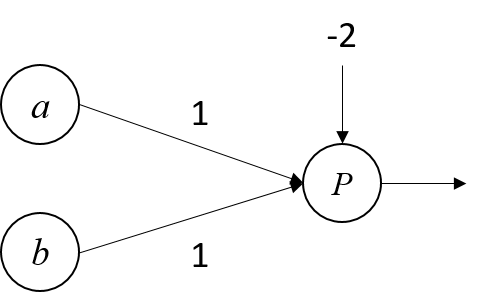
\includegraphics[scale=0.5]{assets/and-perceptron}
  \caption{Fonction ET logique.}
  \label{fig:and-perceptron}
\end{figure}

De même, en prenant $w = (-2, -2)$ et $b = 3$, on code la fonction NAND 
(négation du ET logique). Pour s'en convaincre, on peut dresser le tableau 
des sorties en fonction de toutes les entrées possibles comme cela est fait 
dans la table \ref{table:nand-perceptron}.

\begin{table}[h]
  \centering
\begin{tabular}{|c|c|c|c|}
\hline
$x_1$ & $x_2$ & $wx + b$ & Sortie \\
\hline
0     & 0     & 3        & 1 \\  
0     & 1     & 1        & 1 \\  
1     & 0     & 1        & 1 \\  
0     & 0     & -1       & 0 \\   
\hline
\end{tabular} 
  \caption{Table de vérité du perceptron.}
  \label{table:nand-perceptron}
\end{table}

\begin{figure}[h]
  \centering
  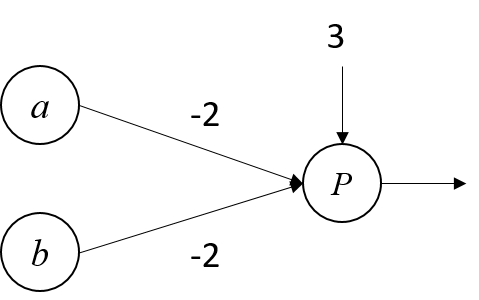
\includegraphics[scale=0.5]{assets/nand-perceptron}
  \caption{Fonction NAND.}
  \label{fig:nand-perceptron}
\end{figure}

Comme la fonction NAND permet de coder n'importe quelle fonction logique, 
on en déduit qu'en utilisant la sortie de perceptrons comme entrées d'autres 
perceptrons, on peut construire n'importe quelle fonction logique.

Cette idée d'empiler des couches de perceptrons pour coder une fonction logique 
conduit naturellement à l'idée que l'on pourrait se faire d'un réseau de neurones.

\begin{figure}[h]
  \centering
  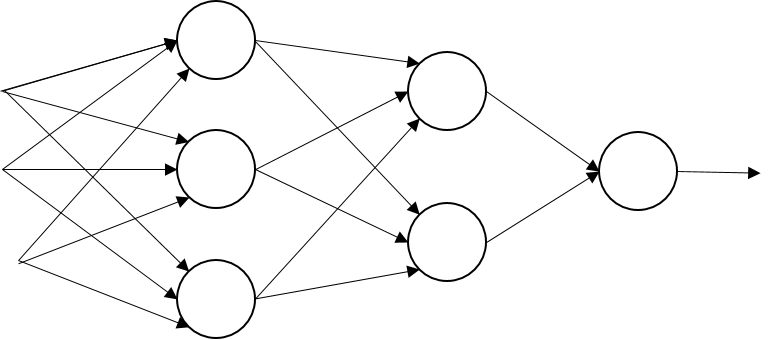
\includegraphics[scale=0.5]{assets/perceptron-network}
  \caption{Un réseau de perceptrons.}
  \label{fig:perceptron-network}
\end{figure}

Jusqu'à présent, nous nous sommes restreint à des entrées binaires (0 ou 1) 
codant des valeurs logiques. Ceci n'est pas nécessaire : les entrées d'un perceptron 
peuvent très bien être des réels.
Plaçons nous, pour les exemples qui vont suivres, dans $\mathbb{R}^2$. 
Pour chaque point $(x, y)$ du plan, on donnera $x$ comme première entrée d'un 
perceptron et $y$ comme seconde entrée. 
Le perceptron ayant pour paramètres $w=(\alpha_x, \alpha_y)$ et $b$ va alors 
séparer l'espace en deux plans par la droite d'équation $\alpha_y y + \alpha_x x + b = 0$. 
Les points tels que $\alpha_y y + \alpha_x x + b \geq 0$ auront pour sortie $1$, et 
les autres auront pour sortie $0$.

Ceci est illustré par la figure \ref{fig:perceptron-example1} dans laquelle la 
partie verte correspond à une sortie positive du perceptron dès lors que $y \geq x$.

\begin{figure}[h]
  \centering
  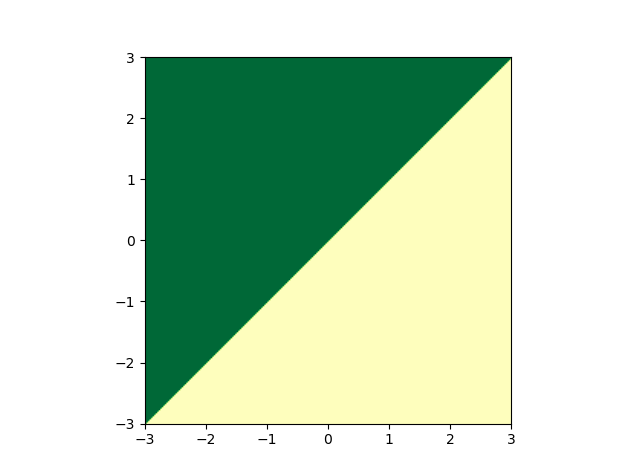
\includegraphics[scale=0.5]{assets/perceptron-example1}
  \caption{Découpage du plan en deux par un perceptron.}
  \label{fig:perceptron-example1}
\end{figure}


En utilisant plusieurs perceptron, on va pouvoir effectuer plusieurs sous-découpage 
de l'espace, et en utilisant un ET logique dans une dernière couche 
on va pouvoir récuperer la partie de l'espace 
correspondant à l'intersection de toutes les parties correspondants aux sorties 
positives des perceptrons de la couche précédente.

\begin{figure}[h]
  \centering
  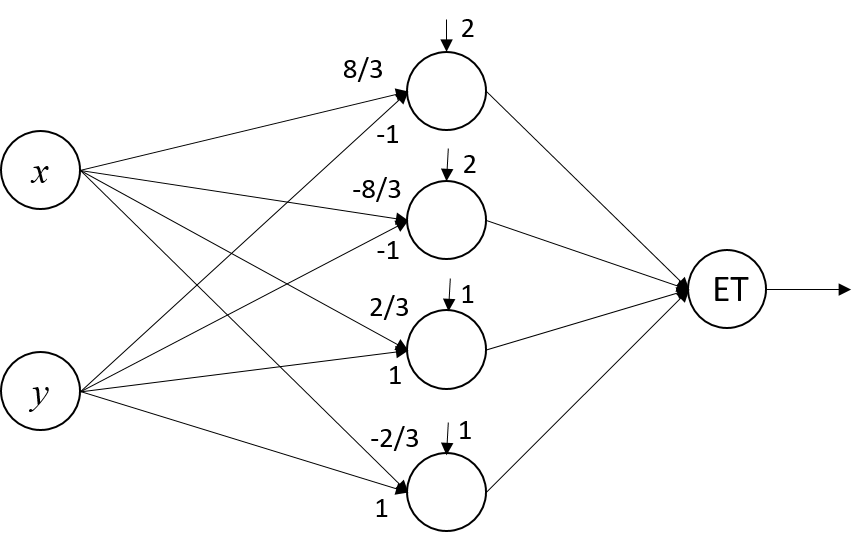
\includegraphics[scale=0.5]{assets/perceptron-network-example2}
  \caption{Un premier réseau de perceptrons.}
  \label{fig:perceptron-network-example2}
\end{figure}

\begin{figure}[h]
  \centering
  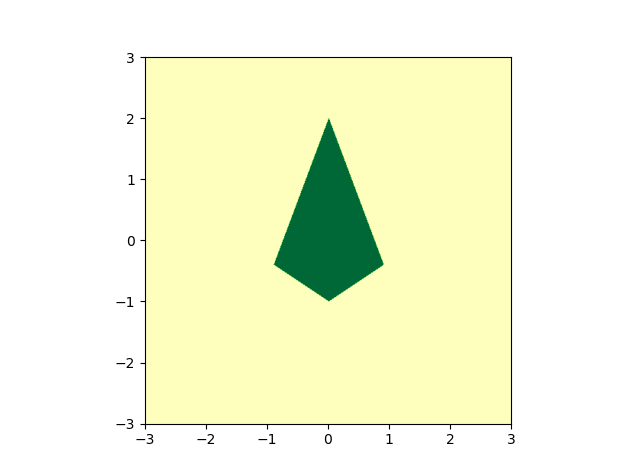
\includegraphics[scale=0.5]{assets/perceptron-example2}
  \caption{Découpage du plan par un réseau de perceptrons.}
  \label{fig:perceptron-example2}
\end{figure}

Cette approche a ses limites car elle ne permet d'obtenir qu'une partie convexe 
du plan. Pour obtenir des parties plus complexes (e.g.\/ non convexes, ou non 
fortement connexes), on peut utiliser d'autres fonctions logiques, comme le OU. 

\begin{figure}[h]
  \centering
  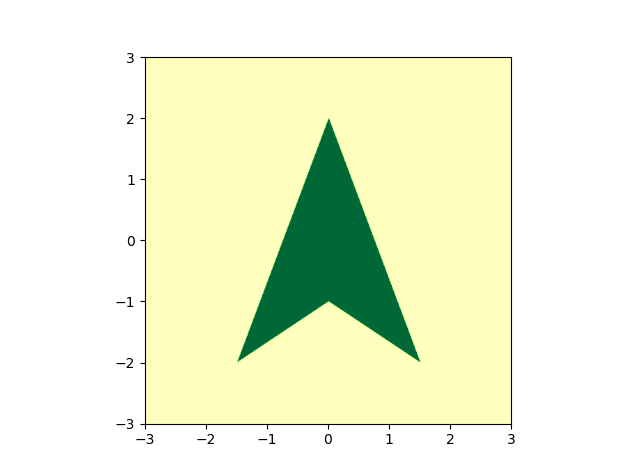
\includegraphics[scale=0.5]{assets/perceptron-example3}
  \caption{Un découpage non convexe du plan avec un réseau de perceptrons à deux couches.}
  \label{fig:perceptron-example3}
\end{figure}

Il n'est pas difficile d'imaginer que l'on puisse étendre ce que l'on vient de faire en 
2 dimensions à un nombre plus grand de dimensions; et avec non plus une seule sortie 
mais plusieurs (correspondant par exemple chacune à une classe, à un chiffre que l'on 
souhaite reonnaître).
On pourrait donc en théorie construire un réseau de neurones avec des perceptrons 
qui serait capable de reconnaître des chiffres. 
L'un des problèmes de cette approche est qu'il faudrait déjà connaître les coefficients 
(ou paramètres) de l'ensemble des perceptrons du réseau.
On pourrait alors avoir envie d'écrire un algorithme permettant de construire un tel 
réseau. On peut imaginer plusieurs principes pour cet algorithme :

\begin{enumerate}
  \item tester tous les coefficients possibles pour les perceptrons;
  \item partir d'une configuration aléatoire et modifier petit à petit les coefficients 
        jusqu'à obtenir un résultat satisfaisant.
\end{enumerate}

La première idée est tout simplement irréalisable car il y a une infinité de valeurs 
possibles pour chaque coefficient du réseau. On pourrait penser à prendre une 
approche probabiliste en testant un certain nombre de réseaux et en espérant tomber sur 
un bon; ce qui paraît néanmoins très improbable ! 
La deuxième idée n'est également pas envisageable car elle souffre d'un problème difficile 
à gérer. La discontinuité de la fonction de Heaviside fait qu'un petit changement de coefficient 
peut faire passer la sortie d'un neurone de 0 à 1 ce qui peut correspondre à un changement 
significatif de l'entrée des neurones de la couche suivante. Il est donc compliqué d'évaluer 
l'impact d'un changement à une couche donnée sur les couches qui suivent.

L'idée qui va être explorée dans les paragraphes suivants est d'utiliser une autre fonction, 
appelée fonction d'activation, que la fonction échelon d'Heaviside; et de faire en sorte que 
cette fonction d'activation soit dérivable (et donc continue) pour pouvoir utiliser des 
résultats d'analyse et pouvoir ainsi estimer l'impact du changement d'un coefficient.
On sera alors en mesure de modifier un réseau généré aléatoirement pour le faire résoudre 
notre problème de classification (on parlera d'apprentissage).



\section{Structure des réseaux de neurones}



\begin{definition}[Fonction sigmoïde]
On appelle fonction sigmoïde la fonction définie de $\mathbb{R}$ dans $[0, 1]$ par :
\[
\sigma(x) = \frac{1}{1 + e^{-x}}
\]
\end{definition}

On notera que $\lim_{x \to +\infty} \sigma(x) = 1$ et $\lim_{x \to -\infty} \sigma(x) = 0$. 
Ainsi, asymptotiquement, la fonction sigmoïde a le même comportement que la fonction 
de Heaviside.

Entre les deux, on a un comportement qui diffère fortement du perceptron avec notamment 
la non discontinuité en 0 et $\sigma(0) = \frac{1}{2}$. 
Dans le cadre de notre utilisation pour la classification on aura tendance 
à considérer que la sortie du neurone est à \textsc{vrai} dès qu'elle sera supérieure 
à une certaine valeur (typiquement $\frac{1}{2}$).

On a également quelques propriétés intéressantes de symétrie. En effet,

\[
\sigma'(x) = \frac{e^{-x}}{1 + e^{-x}} = \sigma(x) (1 - \sigma(x))
\]

\[
\sigma'(x) - \sigma'(-x) = \frac{e^{-x}(e^{2x} + 2 e^{x} + 1) - e^{x}(e^{-2x} + 2 e^{-x} + 1)}{(1+e^{-x})^2 (1+e^{x})^2} = 0
\]

ce qui signifie que la sigmoïde admet pour centre de symétrie le point $(0, \frac{1}{2})$.

Cette fonction a de plus l'avantage d'être dérivable en tout point (et de dérivée non nulle), 
ce qui nous servira plus tard dans le cadre de l'apprentissage.


\begin{definition}[Modélisation d'un neurone]
En notant $b$ le biais du neurone, $w$ son vecteur des poids et $\sigma$ sa fonction 
d'activation, on peut écrire la sortie $a$ d'un neurone en fonction de son entrée $x$ 
de la manière suivante:
\[
a = \sigma(w \cdot x + b)
\]
\end{definition}


\begin{definition}[Vectorisation d'une fonction]
Soit $f$ une fonction de $\mathbb{R} \mapsto \mathbb{R}$. 
On pose pour tout vecteur $x$ de $\mathbb{R}^n$ :
\[
f(x) = 
\begin{pmatrix}
f(x_1) \\
f(x_2) \\
\vdots \\
f(x_n)
\end{pmatrix}
\]
On dit que l'on vectorise la fonction $f$.
\end{definition}

\textbf{Achtung !} Par abus de notation, on utilise encore le nom de $f$ pour désigner 
cette fonction, mais il s'agit bien d'une fonction différente puisqu'elle est à valeurs 
de $\mathbb{R}^n$ dans $\mathbb{R}^n$. Cet abus nous est néanmoins utile pour définir 
simplement les couches d'un réseau de neurones.

On considère dans les définitions suivantes une couche d'un réseau de neurones 
constituée de $n$ neurones. On note $w_i$ le vecteur des poids associé à chaque neurone.
On a alors la définition suivante:
 
\begin{definition}[Matrice des poids]
En notant $w_i$ les vecteurs des poids de $n$ neurones, on définit par blocs 
la matrice $w$ des poids:
\[
w = 
\begin{pmatrix}
{w_1}^T \\
{w_2}^T \\
\vdots \\
{w_n}^T
\end{pmatrix}
\]
\end{definition}

On définit de manière analogue un vecteur des biais.

\begin{definition}[Vecteur des biais]
En notant $b_i$ les biais de $n$ neurones, on définit le vecteur des biais 
d'une couche d'un réseau de neurones par:
\[
b = 
\begin{pmatrix}
{b_1} \\
{b_2} \\
\vdots \\
{b_n}
\end{pmatrix}
\]
\end{definition}

On a alors la proposition suivante:

\begin{proposition}[Ecriture matricielle d'une couche]
Soit une couche d'un réseau constituée de $n$ neurones et ayant pour matrice 
des poids $w$ et pour vecteur des biais $b$. Si les neurones ont tous la même 
fonction d'activation $\sigma$, on peut écrire les sorties des neurones sous la 
forme d'un vecteur $a$ vérifiant:
\[
a = \sigma(w \cdot x + b)
\]
où les $a_i$ correspondent à la sortie du neurone $i$.
\end{proposition}

On notera que dans cette proposition, on utilise la version vectorisée de $\sigma$.
Une écriture équivalente est:
\[
\begin{pmatrix}
  a_1 \\
  a_2 \\
  \vdots \\
  a_n
\end{pmatrix}
 = 
\begin{pmatrix}
  \sigma(w_1 \cdot x + b_1) \\
  \sigma(w_2 \cdot x + b_2) \\
  \vdots \\
  \sigma(w_n \cdot x + b_n)
\end{pmatrix}
\]

En fait, cette écriture est identique à celle d'un unique neurone !
Elle est également intéressante d'un point de vue computationnelle : au lieu 
de calculer une à une les sorties des neurones, il est plus efficace de faire 
un calcul matriciel (les bibliothèques étant en général optimisées pour cela).
Cela permet également d'avoir un code plus simple (avec notamment moins de boucles).

Cette écriture permet également d'écrire de manière très condensée un réseau 
de neurones à plusieurs couches. 
En notant $w^{1}, w^{2}, \cdots, w^{L}$ les matrices de poids de $L$ couches de 
neurones, et $b^{1}, b^{2}, \cdots, b^{L}$ les vecteurs des biais associés, et 
en supposant que tous les neurones ont pour fonction d'activation $\sigma$, on a
\begin{equation}
\label{eq:condensed-multilayer-expression}
a = \sigma(b^{L} + w^{L} \cdot \sigma(b^{L-1} + w^{L-1} \cdot \sigma(\cdots)))
\end{equation}

Pour avoir une écriture plus lisible, on introduit la notion suivante qui 
permet de parler de la sortie pour toute couche:
\begin{definition}[Activation d'un neurone]
On appellera activation du neurone $j$ de la couche $l$ la quantité $a_{j}^{l}$ 
définie par:
\[
a_{j}^{l} = \sigma \left( \sum_{k} w_{jk}^{l} a_{k}^{l-1} + b_{j}^{l} \right)
\]
Il s'agit simplement de la sortie de ce neurone.
\end{definition}

On peut alors réécrire l'équation \ref{eq:condensed-multilayer-expression} de la 
manière suivante, la sortie du réseau étant le vecteur $a^{L}$.
\[
\begin{cases}
 a^{l} = \sigma(w^{l} \cdot a^{l-1} + b^{l}) \\
 a^{0} = x \\
\end{cases}
\]

On constate donc que l'on peut très facilement calculer la sortie d'un réseau 
de neurones par un algorithme itératif. 

Autre remarque importante: il n'est pas nécessaire que les $(w^{l})_{l \in \llbracket 1, L \rrbracket}$ 
aient les mêmes dimensions. Autrement dit, il peut y avoir un nombre différent 
de neurones dans chaque couche; le seule impératif est que les dimensions 
d'une couche à la suivante soient cohérentes.

En reprenant les notations précédentes, on a que $w_{jk}^{l}$ est le poids de la 
connexion reliant le $k$\textsuperscript{ème} neurone de la couche $(l-1)$ au 
$j$\textsuperscript{ème} neurone de la couche $l$.
De la même manière, $b_{j}^{l}$ est le biais du $j$\textsuperscript{ème} neurone 
de la couche $l$.



\section{Apprentissage par la descente de gradient}


On considère dans cette partie un réseau de neurones à $L$ couches, et on note 
encore $w^{1}, w^{2}, \cdots, w^{L}$ les matrices des poids et $b^{1}, \cdots, b^{L}$
les vecteurs des biais. 
On cherche dans cette partie à améliorer de manière itérative la valeur des 
coefficients du réseau pour améliorer les prédictions. 
On introduit pour cela une fonction de coût, croissante de l'erreur, et 
on se ramène à un problème d'optimisation.

\begin{definition}[Fonction de coût quadratique]
Soit $X$ un ensemble d'apprentissage de cardinal $n$. 
On note $a^{L}(x)$ la sortie du réseau de neurones pour l'entrée $x \in X$ et 
$y_{x}$ la sortie désirée. On définit la fonction de coût par:
\[
C(w, b) = \frac{1}{2n} \sum_{x} \vecnorm{y_{x} - a^{L}(x)}^2
\]
\end{definition}

On parle aussi de \textsc{MSE} pour \nfw{mean square error}.

Par la suite, et pour alléger les notations, on écrira souvent $a^{L}$ et $y$ 
au lieu de $a^{L}(x)$ et $y_x$.

Cette fonction a le bon goût d'être convexe. Ainsi, on peut la minimiser en annulant 
sa dérivée. 
Cependant cette fonction dépend de tous les $w^{l}$ et $b^{l}$ ainsi que de la fonction 
$\sigma$, le calcul de la dérivée et de son point d'annulation n'est donc pas facile.
C'est pourquoi on va opter pour un algorithme itératif qui, partant d'un point quelconque 
(i.e.\/ un couple $(w,b)$ donné), va progressivement s'approcher de la solution. 

L'un des algorithmes les plus simples est celui de la descente de gradient.
Partant d'un point $v = (w,b)$, on souhaite trouver $\Delta v$ telle que 
$C(v + \Delta v) \leq C(v)$. Cet algorithme propose de prendre 
$\Delta v = -\eta\nabla C(v)$ avec $\eta$ suffisament petit pour que 
l'on puisse s'assurer de diminuer le coût $C$ et suffisament grand pour que les 
effets soient significatifs.

L'algorithme peut donc se résumer sous la forme suivante:
\begin{enumerate}
  \item étant donné $v = (w, b)$, calculer $\nabla C(v)$;
  \item calculer $v' = v - \eta \nabla C(v)$;
  \item recommencer l'étape 1 avec $v'$.
\end{enumerate}
On itère jusqu'à ce que le coût soit proche de son minimum.

En pratique on utilisera une variante stochastique de l'algorithme. 
En effet, 
\[
C = \frac{1}{n} \sum_{x} C_x \qquad \text{avec} \quad C_x = \frac{1}{2} \vecnorm{y - a^{L}}^2
\]
sera d'autant plus long à calculer que $n$ (la taille de l'échantillon d'apprentissage) 
est grand.
C'est pourquoi on tirera $m < n$ entrées au hasard et on se contentera de calculer 
le coût et son gradient sur ce sous-échantillon.



\section{L'algorithme de rétro-propagation}


L'algorithme de descente de gradient évoqué précédemment est en principe 
très simple. Cependant, le calcul de $\nabla C(v)$ est loin d'être simple. 
Cette quantité dépend en effet de tous les $w_{jk}^{l}$ et les $b_{j}^{l}$.
On présente dans cette partie une manière simple de calculer cette quantité 
via l'algorithme de rétro-propagation. 
Il est cependant nécessaire d'introduire d'abord quelques quantités utiles.


\begin{definition}[Entrées pondérées d'un neurone]
On notera $z_{j}^{l}$ les entrées pondérées du neurone $j$ de la couche $l$.
\[
z_{j}^{l} = \sum_{k} w_{jk}^{l} a_{k}^{l-1} + b_{j}^{l}
\]
\end{definition}

De manière évidente, on a $a_{j}^{l} = \sigma(z_{j}^{l})$.


Comme on l'a vu dans la partie précédente, le coût $C$ s'écrit comme somme 
de coûts unitaires:
\[
C = \frac{1}{n} \sum_{x} C_x
\]
Dans cette partie, on s'intéressa seulement au calcul de la quantité $C_x$ pour un $x$ donné. 
La vrai coût $C$ et $\nabla C$ se calculant simplement en faisant la somme.
On se fixe donc un $x$ et, pour simplifier les notations, on notera $y = y_x$ 
la sortie voulu et $C = C_x$.

L'idée de l'algorithme de rétro-propagation est de partir d'une quantité que 
l'on peut facilement calculer à partir de la sortie du réseau (que l'on obtient 
en faisant un \nfw{feedforward}, c'est à dire en parcourant le réseau depuis la 
première couche jusqu'à la dernière) et de revenir en arrière (\nfw{backpropagation}) 
pour attribuer à chaque coefficient du réseau une part de l'erreur.

Notons $a^L$ la sortie du réseau, on a:
\[
C = \frac{1}{2} \vecnorm{y - a^L}^2 = \frac{1}{2} \sum_{j} (y_j - a_{j}^{L})^2
\]
On obtient donc très facilement le résultat suivant.
\[
\frac{\partial C}{\partial a_{j}^{L}} = (a_{j}^{L} - y_j)
\]
Que l'on écrira sous forme vectorielle.
\[
\nabla_a C = a^{L} - y 
\]

La principe de l'algorithme de rétro-propagation va être de partir de cette 
quantité et de parcourir les couches du réseau à l'envers pour calculer les 
dérivées partielles $\frac{\partial C}{\partial w_{jk}^{l}}$ et $\frac{\partial C}{\partial b_{j}^{l}}$.

\begin{definition}[Erreur d'un neurone]
On définit l'erreur au neurone $j$ de la couche $l$ par:
\[
\delta_{j}^{l} = \frac{\partial C}{\partial z_{j}^{l}}
\]
\end{definition}

Cette définition est posée de manière un peu arbitraire et permet simplement 
de simplifier l'écriture des calculs que nous ferrons plus tard. 
Une autre définition possible aurait été de prendre l'erreur comme étant égale 
à $\frac{\partial C}{\partial a_{j}^{l}}$. Cela ne change pas grand chose car on 
a la relation suivante (règle de la chaîne).

\[
\frac{\partial C}{\partial z_{j}^{l}} = \sum_{i} \frac{\partial C}{\partial a_{i}^{l}} \frac{\partial a_{i}^{l}}{\partial z_{j}^{l}}
= \sum_{i} \frac{\partial C}{\partial a_{i}^{l}} \frac{\partial \sigma(z_{i}^{l})}{\partial z_{j}^{l}} = \frac{\partial C}{\partial a_{j}^{l}} \sigma'(z_{j}^{l})
\]


\begin{definition}[Produit de Hadamard]
Soit $S$ et $T$ deux matrices (ou vecteurs) de même dimension, on appelle 
produit de Hadamard de $S$ et $T$, noté $S \odot T$ la matrice de même dimension 
que $T$ et donc les composantes sont les produits éléments par éléments des 
coefficients de $S$ et $T$, i.e.\/
\[
(S \odot T)_{ij} = S_{ij} \times T_{ij}
\]
\end{definition}



\begin{proposition}[Equations de la rétro-propagation]
On a les relations suivantes: \\
Erreur au niveau de la dernière couche: 
\begin{equation}
  \label{eq:bp1}
\delta^{L} = \nabla_{a} C \odot \sigma'(z^{L})
\end{equation}
Erreur au niveau de la couche $l$:
\begin{equation}
  \label{eq:bp2}
\delta^{l} = ((w^{l+1})^T \delta^{l+1}) \odot \sigma'(z^{l})
\end{equation}
Dérivées partielles par rapport aux biais:
\begin{equation}
  \label{eq:bp3}
\frac{\partial C}{\partial b_{j}^{l}} = \delta_{j}^{l}
\end{equation}
Dérivées partielles par rapport aux poids:
\begin{equation}
  \label{eq:bp4}
\frac{\partial C}{\partial w_{jk}^{l}} = a_{k}^{l-1} \delta_{j}^{l}
\end{equation}
\end{proposition}

Ces équations nous donnent une méthode simple pour calculer les dérivées partielles 
par rapport aux coefficients du réseau et permettent ainsi d'appliquer la méthode 
de la descente de gradient.

\begin{proof}[Preuve de l'équation \ref{eq:bp1}]
Il suffit de reprendre ce que l'on a fait précédemment (règle de la chaîne). 
\[
\delta_{j}^{L} = \frac{\partial C}{\partial z_{j}^{L}} =
 \sum_{i} \frac{\partial C}{\partial a_{i}^{L}} \frac{\partial a_{i}^{L}}{z_{j}^{L}} =
 \sum_{i} \frac{\partial C}{\partial a_{i}^{L}} \frac{\partial \sigma(z_{i}^{L})}{z_{j}^{L}} =
 \frac{\partial C}{\partial a_{j}^{L}} \sigma'(z_{j}^{L})
\]
Soit sous forme vectorielle,
\[
\delta^{L} = \frac{\partial C}{\partial a^{L}} \odot \sigma'(z^{L})
\]
quantité que l'on écrit $\nabla_{a} C \odot \sigma'(z^{L})$.
\end{proof}

\vspace{1em}

Le résultat \ref{eq:bp2} est certainement le plus intéressant car c'est lui qui permet 
de remonter le réseau pour attribuer les erreurs aux différentes couches. 
Il dit grossièrement que pour retrouver l'erreur à la couche $l$, il suffit 
d'appliquer la transposée de la matrice de poids de la couche $l+1$ à l'erreur 
sur cette même couche et de multiplier par la dérivée de la sigmoïde.

\begin{proof}[Preuve de l'équation \ref{eq:bp2}]
On applique un raisonnement similaire à la preuve précédente.
\begin{align}
  \delta_{j}^{l} &= \frac{\partial C}{\partial z_{j}^{l}} \\
                 &= \sum_{k} \frac{\partial C}{\partial z_{k}^{l+1}} \frac{\partial z_{k}^{l+1}}{\partial z_{j}^{l}} \\
				 &= \sum_{k} \frac{\partial z_{k}^{l+1}}{\partial z_{j}^{l}} \delta_{k}^{l+1}
\end{align}
On se remémore ensuite l'expression de $z_{k}^{l+1}$:
\[
z_{k}^{l+1} = \sum_{i} w_{ki}^{l+1} a_{i}^{l} + b_{k}^{l+1} = \sum_{i} w_{ki}^{l+1} \sigma(z_{i}^{l}) + b_{k}^{l+1}
\]
Ce qui nous permet d'obtenir
\[
\frac{\partial z_{k}^{l+1}}{\partial z_{j}^{l}} = w_{kj}^{l+1} \sigma'(z_{j}^{l})
\]
On obtient donc le résultat voulu
\[
\delta_{j}^{l} = \sum_{k} w_{kj}^{l+1} \delta_{k}^{l+1} \sigma'(z_{j}^{l})
\]
\end{proof}

\vspace{1em}

Les deux derniers résultats servent à relier les quantités calculées aux 
quantités voulues.

\begin{proof}[Preuve de l'équation \ref{eq:bp3}]
\[
\frac{\partial C}{\partial b_{j}^{l}} =
 \sum_{i} \frac{\partial C}{\partial z_{i}^{l}} \frac{\partial z_{i}^{l}}{\partial b_{j}^{l}} =
 \frac{\partial C}{\partial z_{j}^{l}} \frac{\partial z_{j}^{l}}{\partial b_{j}^{l}}
\]
Or on sait que $z_{j}^{l} = \sum_{k} w_{jk}^{l} a_{k}^{l-1} + b_{j}^{l}$ donc la deuxième dérivée vaut $1$.
Au final,
\[
\frac{\partial C}{\partial b_{j}^{l}} = \frac{\partial C}{\partial z_{j}^{l}} = \delta_{j}^{l}
\]
\end{proof}

\begin{proof}[Preuve de l'équation \ref{eq:bp4}]
$z_{j}^{l} = \sum_{i} w_{ji}^{l} a_{i}^{l-1} + b_{j}^{l}$ donc $\frac{\partial z_{j}^{l}}{\partial w_{jk}^{l}} = a_{k}^{l-1}$.
Ainsi, 
\[
\frac{\partial C}{\partial w_{jk}^{l}} = a_{k}^{l-1} \delta_{j}^{l}
\]
\end{proof}



\section{Reconnaissance avec un réseau de neurone}

Dans cette partie, on se propose d'utiliser ce que l'on a vu 
précédement pour construire un réseau de neurones permettant 
de répondre à notre problème de classification.


\subsection{Construction du réseau de neurones}

On se propose de construire un réseau de neurones ayant une 
seule couche cachée contenant $p$ neurones. 
Les couches d'entrées et de sorties contiennent respectivement 
$28 \times 28 = 784$ et 10 neurones.

Chaque neurone de la couche de sortie correspond à une classe 
(de 0 à 9) et on dira que le réseau classe une entrée dans la 
classe $C_i$ si la sortie $i$ est la plus élevée.

On rappelle que puisqu'on utilise comme fonction d'activation 
la sigmoïde, les sorties sont toutes positives.


\subsection{Apprentissage}

Les images du jeu d'entraînement de \textsc{MNIST} sont des 
tableaux de 28 par 28 contenant des entiers de 0 à 255.
On commence par redimensionner le tableau en un vecteur 
de taille 784 que l'on divise ensuite par 255 pour obtenir 
des composantes entre 0 et 1. 
Cela n'est pas nécessaire dans l'absolu mais donne de 
meilleurs résultats en pratique.
En effet, la sigmoïde faisant intervenir une exponentielle, 
on aura du mal à calculer numériquement $e^{-255}$.

Pour les sorties, on convertit les différentes étiquettes 
en des vecteurs de taille 10 dont toutes les composantes 
sont nulles sauf la composante correspondant à la classe 
qui vaut 1.

On initialise les poids et biais de notre réseau par des 
tirages aléatoires suivant une $\mathcal{N}(0, 1)$.

On découpe la phase d'apprentissage en \nfw{epochs}. 
Comme nous l'avons dit précédemment, on ne cherchera pas 
à calculer la valeur exacte de la dérivée du coût 
pour changer nos coefficients mais seulement une 
approximation de cette dérivée.
On va donc découper de manière aléatoire notre jeu 
d'entraînement en \nfw{mini-batch} (i.e. en sous-échantillon) 
dont l'union fait le jeu complet.
Il s'agit donc en quelque sorte d'une partition du 
jeu de départ créée aléatoirement.
On effectue la descente de gradient avec ces 
\nfw{mini-batchs}. 
Lorsque l'on a utilisé tous les \nfw{mini-batchs}, 
et donc toutes les données, on dit que l'on a 
effectué une \nfw{epoch}.
On peut alors en commencer une autre en effectuant un 
nouveau découpage aléatoire du jeu d'entraînement.


\subsection{Résultats}


En prenant $p = 30$ neurones sur la couche cachée, et 
en prenant des \nfw{mini-batchs} de taille 10, 
on arrive en une trentaine d'\nfw{epochs} et avec 
un taux d'apprentissage $\eta = 3,0$ à un taux de 
reconnaissance d'environ 95\% sur le jeu de test.
